\documentclass{ximera}

\input{../preamble.tex}

\outcome{Solve linear inequalities.}
\outcome{Solve nonlinear inequalities using a sign chart.}

\title[Dig-In:]{Inequalities}
\begin{document}
\begin{abstract}
  We discuss inequalities.
\end{abstract}
\maketitle

Devyn asked what score was needed on the third exam to have an average of 82.  This gave us the equation $\displaystyle \dfrac{74 + 84 + x}{3} = 82$.  
The solutions only tell us what will give an average \emph{exactly} 82.  It may have been more advantageous to ask what score was needed to have an
average of at least 82, yielding not an equation, but an \emph{inequality}, $\displaystyle \dfrac{74+84+x}{3} \geq 82$.

As with equations, there are various types of inequalities.  

A \emph{linear inequality in $x$} is an inequality which is equivalent to  $ax + b >0$, $ax + b \geq 0$, $ax+b < 0$, or $ax + b \leq 0$.
We solve the inequality in much the same manner as with a linear equation.  The main differences come from changing the direction of the inequality when multiplying/dividing
by a negative quantity and expressing our answers in interval notation.

\begin{example}
 	Solve the inequality $\displaystyle \dfrac{2x}{3}-4 < 3\left( 2-x \right)$.
	\begin{explanation}
    		As with equations, we'll start by simplifying and combining like terms.
		\begin{align*}
			\dfrac{2x}{3} -4 &< 3\left( 2-x \right)\\
			\dfrac{2x}{3} - 4 &< 6 - 3x\\
			\dfrac{2x}{3}+3x &< 6 + 4\\
			\dfrac{11}{3} x &< 10\\
			x &< \dfrac{30}{11}
		\end{align*}
		All $x$ less than $\frac{30}{11}$ satisfy the inequality.
		
		The solution is $\left( -\infty , \dfrac{30}{11} \right)$.
	\end{explanation}
\end{example}

Nonlinear inequalities are more complicated.  To solve them, we will use a tool called a \emph{sign chart}.
The process requires us to move all the nonzero terms of the inequality to one side, and factor.
\begin{example}
	Solve the inequality \[ \dfrac{x^3 \left(2x-5\right)^2}{x+1} > 0.\]

	\begin{explanation}
		Since the right-hand side is zero, we are really asking where the left-hand side will be positive.  The only way
		a nice formula like the left-hand side can switch from positive to negative, or vice-versa, is if it is either zero
		or undefined at the point where it changes.

		Notice where the left-hand side would be either zero or undefined.  Those occur at $x = -1, 0, \frac{5}{2}$.  
		We'll use those points to split the number line into four regions. Inside each of those regions, our factors are either
		always positive or always negative.
		
		\begin{tikzpicture} 
			\tkzTabInit[lgt=2,espcl=1] 
				{$x$         /1, 
				$x^3$   /1, 
				$\left(2x-5\right)^2$  /1,
				$x+1$       /1}% 
				{  , $-1$ , $0$ ,$\dfrac{5}{2}$,  }% 
			\tkzTabLine{ , - , d , - , t , + , t , + ,}
			\tkzTabLine{ , + , d , + , t , + , t , + ,}
			\tkzTabLine{ , - , d , + , t , + , t , +, }
		\end{tikzpicture} 
		
		For $x < -1$, we find $x^3 < 0$, $(2x-5)^2 > 0$, and $x+1 < 0$.  Together, that means the left-hand side of our inequality has the form 
		$\displaystyle \dfrac{ \textrm{negative} \cdot \textrm{positive}}{\textrm{negative}}$.  It is, therefore, positive in that region, and makes up
		part of our solution.  We cannot include the endpoint $x=-1$ in the solution, as the fraction is undefined there.
		
		In the same way, we see that in the intervals $\left( 0, \frac{5}{2} \right)$ and $\left( \frac{5}{2}, 0\right)$, the left-hand side of the inequality is also positive.
		Notice that the inequality is NOT satisfied at $x=\frac{5}{2}$, where the left-hand side equals zero.  
		
		The solution is $\left( -\infty, -1 \right) \cup \left( 0, \frac{5}{2} \right) \cup \left( \frac{5}{2}, \infty \right)$.
	\end{explanation}
\end{example}


\begin{example}
	Solve the inequality \[ \dfrac{2x}{x-1} \leq \dfrac{5-x}{x-1}. \] 

	\begin{explanation}
		Let's start by moving all the terms to one side of the inequality.
		\begin{align*}
			\dfrac{2x}{x-1} &\leq \dfrac{5-x}{x-1}\\
			\dfrac{2x}{x-1} - \dfrac{5-x}{x-1} &\leq 0\\
			\dfrac{3x - 5}{x-1} &\leq 0
		\end{align*}
		\begin{tikzpicture} 
			\tkzTabInit[lgt=2,espcl=1] 
				{$x$         /1, 
				$3x-5$   /1, 
				$x-1$       /1}% 
				{  , $1$ , $\dfrac{5}{3}$,  }% 
			\tkzTabLine{ , - , d , - , t , + ,}
			\tkzTabLine{ , - , d , + , t , + ,}
		\end{tikzpicture} 
		The solution is $\displaystyle \left( 1, \dfrac{5}{3} \right]$.
	\end{explanation}
\end{example}

\begin{problem}
	Find the solution of the inequality \[ \dfrac{x}{x-4} \geq \dfrac{2x-1}{x-4}. \]
	\begin{multipleChoice}
		\choice[correct]{$\left[1, 4\right)$}
		\choice{$\left(-\infty, 1\right] \bigcup \left(4, \infty\right)$}
		\choice{$\left(1, 4\right)$}
		\choice{$\left(-\infty, 1\right) \bigcup \left(4, \infty\right)$}
		\choice{None of the above}
	\end{multipleChoice}
\end{problem}














\end{document}
